\documentclass[11pt,aspectratio=43,ignorenonframetext,t]{beamer}
% Sustainable material selection exercise: comparing two EPDs.
% Based on the University of Manchester beamer template
% (https://github.com/CASSON-LAB/uom_beamer_template); the theme is included
% locally as beamerthemeUoM_alex.sty so the deck compiles offline.
%
% Compile with: lualatex epd_ppt.tex  (fontspec/XeLaTeX or LuaLaTeX required)


%%%%%%%%%%%%%%%%%% DOCUMENT SETUP %%%%%%%%%%%%%%%%%%

\usepackage{fontspec}
  \setmainfont[Ligatures=TeX]{Arial}

\mode<presentation>{
  \usetheme[framenumber,titleframestart=1]{UoM_alex}
  \usefonttheme{professionalfonts} % using non standard fonts for beamer
  \usefonttheme{serif}             % set font to Arial
}


% Packages
\usepackage{graphicx}  % for graphics files
  \graphicspath{ {./images/} {./ref/picture/} }
\usepackage{amsmath}   % assumes amsmath package installed
\usepackage{amssymb}   % assumes amsmath package installed
\usepackage{booktabs}  % professional table rules
\usepackage{tabularx}  % allows fixed width tables
\usepackage{multirow}  % allows merging of rows in tables
\usepackage{array}     % column types for tables
\usepackage{bm}        % allow bold fonts in equations
\usepackage[document]{ragged2e} % left aligned text for accessibility
\usepackage{hyperref}  % add hyperlinks to document
  \hypersetup{
    colorlinks=true,
    linkcolor=uomlinkblue,
    filecolor=uomlinkblue,
    urlcolor=uomlinkblue,
    pdflang={en-GB},
  }

% Custom commands
\newcommand{\fig}[1]{Fig.~\ref{#1}}
\newcommand{\tab}[1]{Table~\ref{#1}}
\newcommand{\degree}{\ensuremath{^\circ}}
\newcolumntype{Z}{>{\centering\arraybackslash}X}  % tabularx centered columns
\newcommand{\ph}[1]{\textit{[#1]}}                 % fill-in placeholder


%%%%%%%%%%%%%%%%%% FRONT MATTER %%%%%%%%%%%%%%%%%%
\title{Environmental Product Declarations in Construction:\\ Mineral Wool vs.\ XPS Insulation}
\subtitle{Which insulation supports a more sustainable decision?}
\author{Group \_\_ \\[0.8ex]
  \small \ph{Name} -- \ph{Student ID} \quad \ph{Name} -- \ph{Student ID} \\[0.3ex]
  \small \ph{Name} -- \ph{Student ID} \quad \ph{Name} -- \ph{Student ID}}
\institute{Course unit: \ph{course code and title} \;|\; The University of Manchester}
\date{\today}

\begin{document}


%%%%%%%%%%%%%%%%%% SLIDE 1: COVER %%%%%%%%%%%%%%%%%%
\begin{frame}
  \titlepage
  \note{
    Cover slide: title of the investigation plus the names and student IDs of
    all four group members. Keep the title specific: name the two products and
    the application they serve (e.g.\ insulation for a cavity wall).
  }
\end{frame}


%%%%%%%%%%%%%%%%%% SLIDE 2: PRODUCTS AND EPDs %%%%%%%%%%%%%%%%%%
\begin{frame}{Products and their EPDs}
  \setbeamertemplate{itemize/enumerate body begin}{\scriptsize}
  \begin{itemize}
    \item \textbf{Product A:} ROCKWOOL \emph{Safe'n'Sound} stone wool batt, ROCKWOOL North America
    \item \textbf{Product B:} URSA XPS NVII L extruded polystyrene board, URSA Insulation S.A.\ (Madrid), Bondeno plant (Italy)
    \item \textbf{Functional unit:} 1\,m$^2$ insulation at a declared thermal resistance --- \alert{not the same value} (A: RSI~1.0; B: $R=1.50$ at 50\,mm); normalised next slide
    \item \textbf{EPD programme:} A: UL Environment (ISO 14025), EPD 4789092768.101.1; B: International EPD\textsuperscript{\textregistered} System S-P-09927 (EN 15804+A2), ver.\ M.\ G\'omez Ferrer
    \item \textbf{System boundary:} cradle-to-grave in both (A: A1--C4; B: A1--A3, A4, A5, B1--B7, C1--C4, plus D)
  \end{itemize}

  \vfill
  \begin{center}
    \setlength{\fboxsep}{2pt}
    \fbox{\parbox[c][1.9cm][c]{0.34\textwidth}{\centering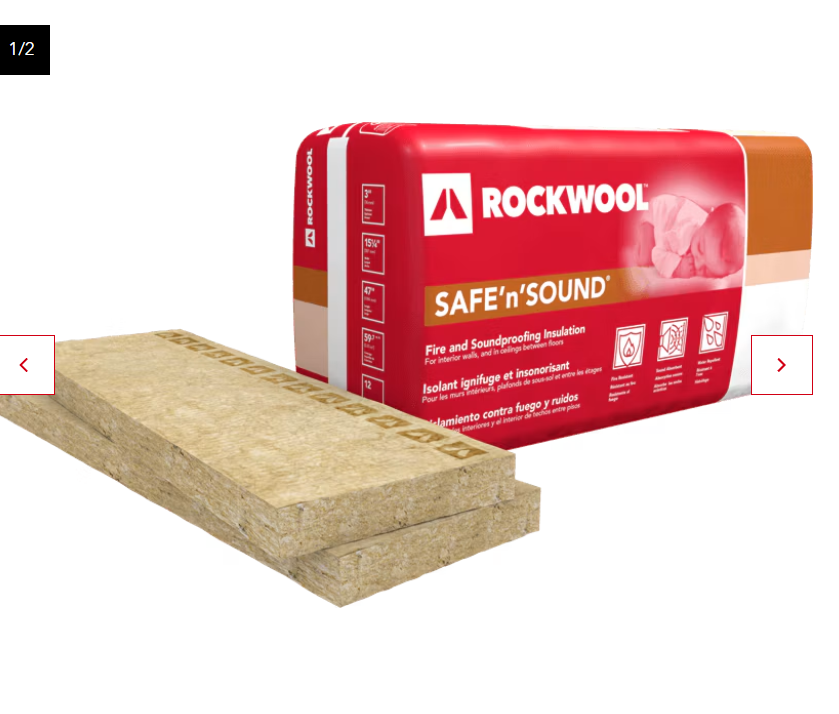
\includegraphics[height=1.6cm]{rockwool1.png}}}\hspace{2em}%
    \fbox{\parbox[c][1.9cm][c]{0.34\textwidth}{\centering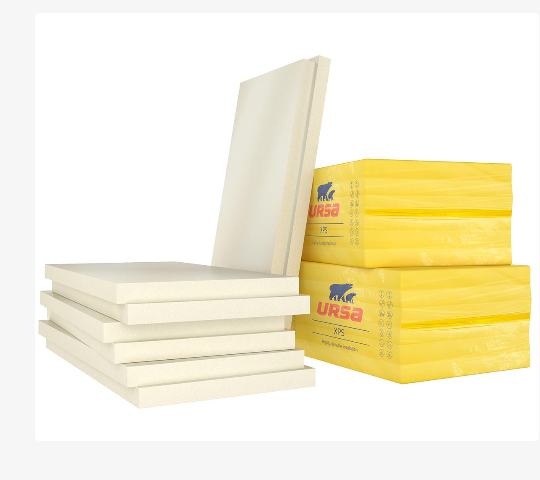
\includegraphics[height=1.6cm]{ursa.png}}}\\[0.4ex]
    {\scriptsize Product images: ROCKWOOL \emph{Safe'n'Sound} (left) and URSA XPS NVII L (right).}
  \end{center}

  \note{
    State only verifiable facts taken from the two EPDs. The functional unit must
    be directly comparable; if it is not, normalise the declared values before
    any comparison. Flag any difference in system boundary here so that the
    reader can interpret the numbers on the next slide correctly.
  }
\end{frame}


%%%%%%%%%%%%%%%%%% SLIDE 3: ENVIRONMENTAL PERFORMANCE %%%%%%%%%%%%%%%%%%
\begin{frame}{Environmental performance comparison}
  \begin{table}
    \centering
    \scriptsize
    \renewcommand{\arraystretch}{1.25}
    \begin{tabularx}{\textwidth}{@{}Z r r@{}}
      \toprule
      \textbf{Indicator (per 1\,m$^2$ of insulation)} & \textbf{Product A} & \textbf{Product B} \\
      & \textbf{(RSI 1.0)} & \textbf{($R = 1.50$)} \\
      \midrule
      GWP-total, A1--A3, as declared              & 1.31 kg CO$_2$e  & 7.01 kg CO$_2$e \\
      GWP-total, A1--A3, scaled to $R = 1.50$     & $\approx$1.97 kg CO$_2$e & 7.01 kg CO$_2$e \\
      GWP-total, A1--C4 (cradle-to-grave)         & 2.03 kg CO$_2$e  & 7.75 kg CO$_2$e \\
      Total non-renewable primary energy, A1--A3  & n.d.             & 136 MJ \\
      Net fresh water use, A1--A3                 & n.d.             & 0.119 m$^3$ \\
      \bottomrule
    \end{tabularx}
    \caption{Declared environmental indicators per functional unit of insulation.}
  \end{table}

  \vspace{0.6ex}
  {\scriptsize Sources: URSA EPD S-P-09927 (A1--A3, 50\,mm, $R=1.50$); ROCKWOOL GWP look-up tables (RSI~1.0). A1--C4 = A1--A3 + A4 + A5 + C2 + C4. n.d. = not declared; scaling to $R=1.50$ assumes proportionality (indicative). BEAM reference, kg CO$_2$e per m$^2$ RSI: mineral wool 3.30, XPS HFC-blown 55.50, low-GWP 4.90.}

  \note{
    Compare only like with like: the two EPDs declare the same functional unit
    conceptually (1 m$^2$ at a stated thermal resistance) but at different
    resistance values, so the scaled row is the fair comparison. Report the
    product-stage values first, then cradle-to-grave, and state explicitly that
    primary energy and water are unavailable for Product A.
  }
\end{frame}


%%%%%%%%%%%%%%%%%% SLIDE 4: INTERPRETING THE RESULTS %%%%%%%%%%%%%%%%%%
\begin{frame}{Interpreting the results}
  \setbeamertemplate{itemize/enumerate body begin}{\footnotesize}
  \begin{itemize}
    \item \textbf{GWP:} mineral wool wins on every basis --- 1.97 vs.\ 7.01 kg CO$_2$e per m$^2$ at $R=1.50$; XPS carries $\approx$3.6$\times$ the product-stage footprint
    \item \textbf{Energy and water:} ranking cannot be checked --- ROCKWOOL's tables publish only GWP, so XPS's 136 MJ and 0.119 m$^3$ cannot be benchmarked yet
    \item \textbf{Magnitude of the gap:} real, but far below the $>$10$\times$ quoted for HFC-blown XPS (55.50 vs.\ 3.30 per RSI); 7.01 indicates a low-GWP blowing agent (type undisclosed)
    \item \textbf{Verdict:} no unconditional winner --- mineral wool is preferable on GWP for interior walls, but other indicators and the application still matter
    \item \textbf{Caveats:} functional units differ (RSI 1.0 vs.\ $R=1.50$), so the scaled row is indicative; different programmes and PCRs limit strict comparability
  \end{itemize}

  \note{
    Interpret rather than repeat the table: say who wins each indicator, how big
    the difference is, and whether it exceeds the uncertainty of the underlying
    data. Do not claim a single winner if the indicators disagree.
  }
\end{frame}


%%%%%%%%%%%%%%%%%% SLIDE 5: COMPARISON AND DECISION %%%%%%%%%%%%%%%%%%
\begin{frame}{Comparison and decision}
  \setbeamertemplate{itemize/enumerate body begin}{\footnotesize}
  \begin{itemize}
    \item \textbf{Recommendation:} specify mineral wool for low-carbon interior partitions; if XPS is required (inverted roofs, below-grade, load-bearing), demand blowing-agent disclosure and prefer low-GWP variants
    \item \textbf{Environmental trade-off:} XPS trades a higher GWP for CS(10/Y)700 compressive strength (700 kPa), moisture resistance and a 50-year service life --- properties mineral wool cannot match structurally
    \item \textbf{Space-efficiency trade-off:} XPS reaches the same $R$-value at $\lambda \approx 0.034$--0.036 W/(m$\cdot$K) in a thinner profile; mineral wool needs more build-up, a hidden cost of its lower GWP
    \item \textbf{Most interesting finding:} ``XPS $=$ high carbon'' is outdated --- low-GWP agents shrink the gap from $>$10$\times$ to $\approx$3.6$\times$; category labels alone cannot drive specification
    \item \textbf{Information still needed:} exact blowing agent; ROCKWOOL primary energy and water; A4 transport distance; fire class and end-of-life --- one indicator is not the whole story
  \end{itemize}

  \note{
    The decision must be justified and limited to what the EPDs actually support.
    A better GWP value does not automatically make a product environmentally
    preferable: service life, module coverage and functional equivalence all
    affect the outcome. State the additional evidence needed before a final
    specification decision.
  }
\end{frame}


%%%%%%%%%%%%%%%%%% SLIDE 6: REFERENCES %%%%%%%%%%%%%%%%%%
\begin{frame}{References}
  \setbeamertemplate{itemize/enumerate body begin}{\scriptsize}
  \begin{itemize}
    \item \textbf{EPD, Product B:} URSA Insulation S.A., \emph{URSA XPS NVII L}, International EPD System, reg.\ S-P-09927 / EPD-IES-0009927:002, 2023 -- \url{https://www.environdec.com/library/epd9927}
    \item \textbf{EPD, Product A:} ROCKWOOL, \emph{Safe'n'Sound}, UL Environment EPD no.\ 4789092768.101.1, GWP look-up tables -- \url{https://www.rockwool.com/siteassets/o2-rockwool/documentation/technical-bulletins/commercial/epd-gwp-look-up-tables.pdf}
    \item \textbf{Database:} One Click LCA, \emph{Stone wool insulation batt, Safe n Sound, Rockwool North America} -- \url{https://materials.oneclicklca.com/en/material/stone-wool-insulation-batt-for-interior-walls/62d145282102db6d5dadbbdd}
    \item \textbf{Standards:} EN 15804:2012+A2:2019, ISO 14025:2006; PCR 2019:14 v1.11 and C-PCR-005 (EN 16783)
    \item \textbf{Background data:} Vermont Public Service Department, \emph{Default Insulation GWP Values} (BEAM); EPDs accessed 23 October 2026
  \end{itemize}

  \note{
    Give full citations and working links to both EPDs, plus the standard that
    governs them and the date the documents were retrieved. Do not cite sources
    that were not used to reach the conclusions.
  }
\end{frame}


%%%%%%%%%%%%%%%%%% END MATTER %%%%%%%%%%%%%%%%%%
\end{document}
